\chapter{Ancillary Representation Analyses Figures}

\section{RNN Architecture Learned Representations}
\label{rnn_architecture_representations}

\section{MLP Architecture Learned Representations}
\label{mlp_architecture_representations}

\section{RNN Architecture with environmental and game events covariates learned representations}
\label{rnn_env_even_architecture_representations}

\subsection{Behavioural Representations}

\subsection{Environmental Representations}

\subsection{Game Events Representations}

\section{Partitions behavioural metrics representations}
\label{partitions_behavioural}

\begin{figure}[ht]
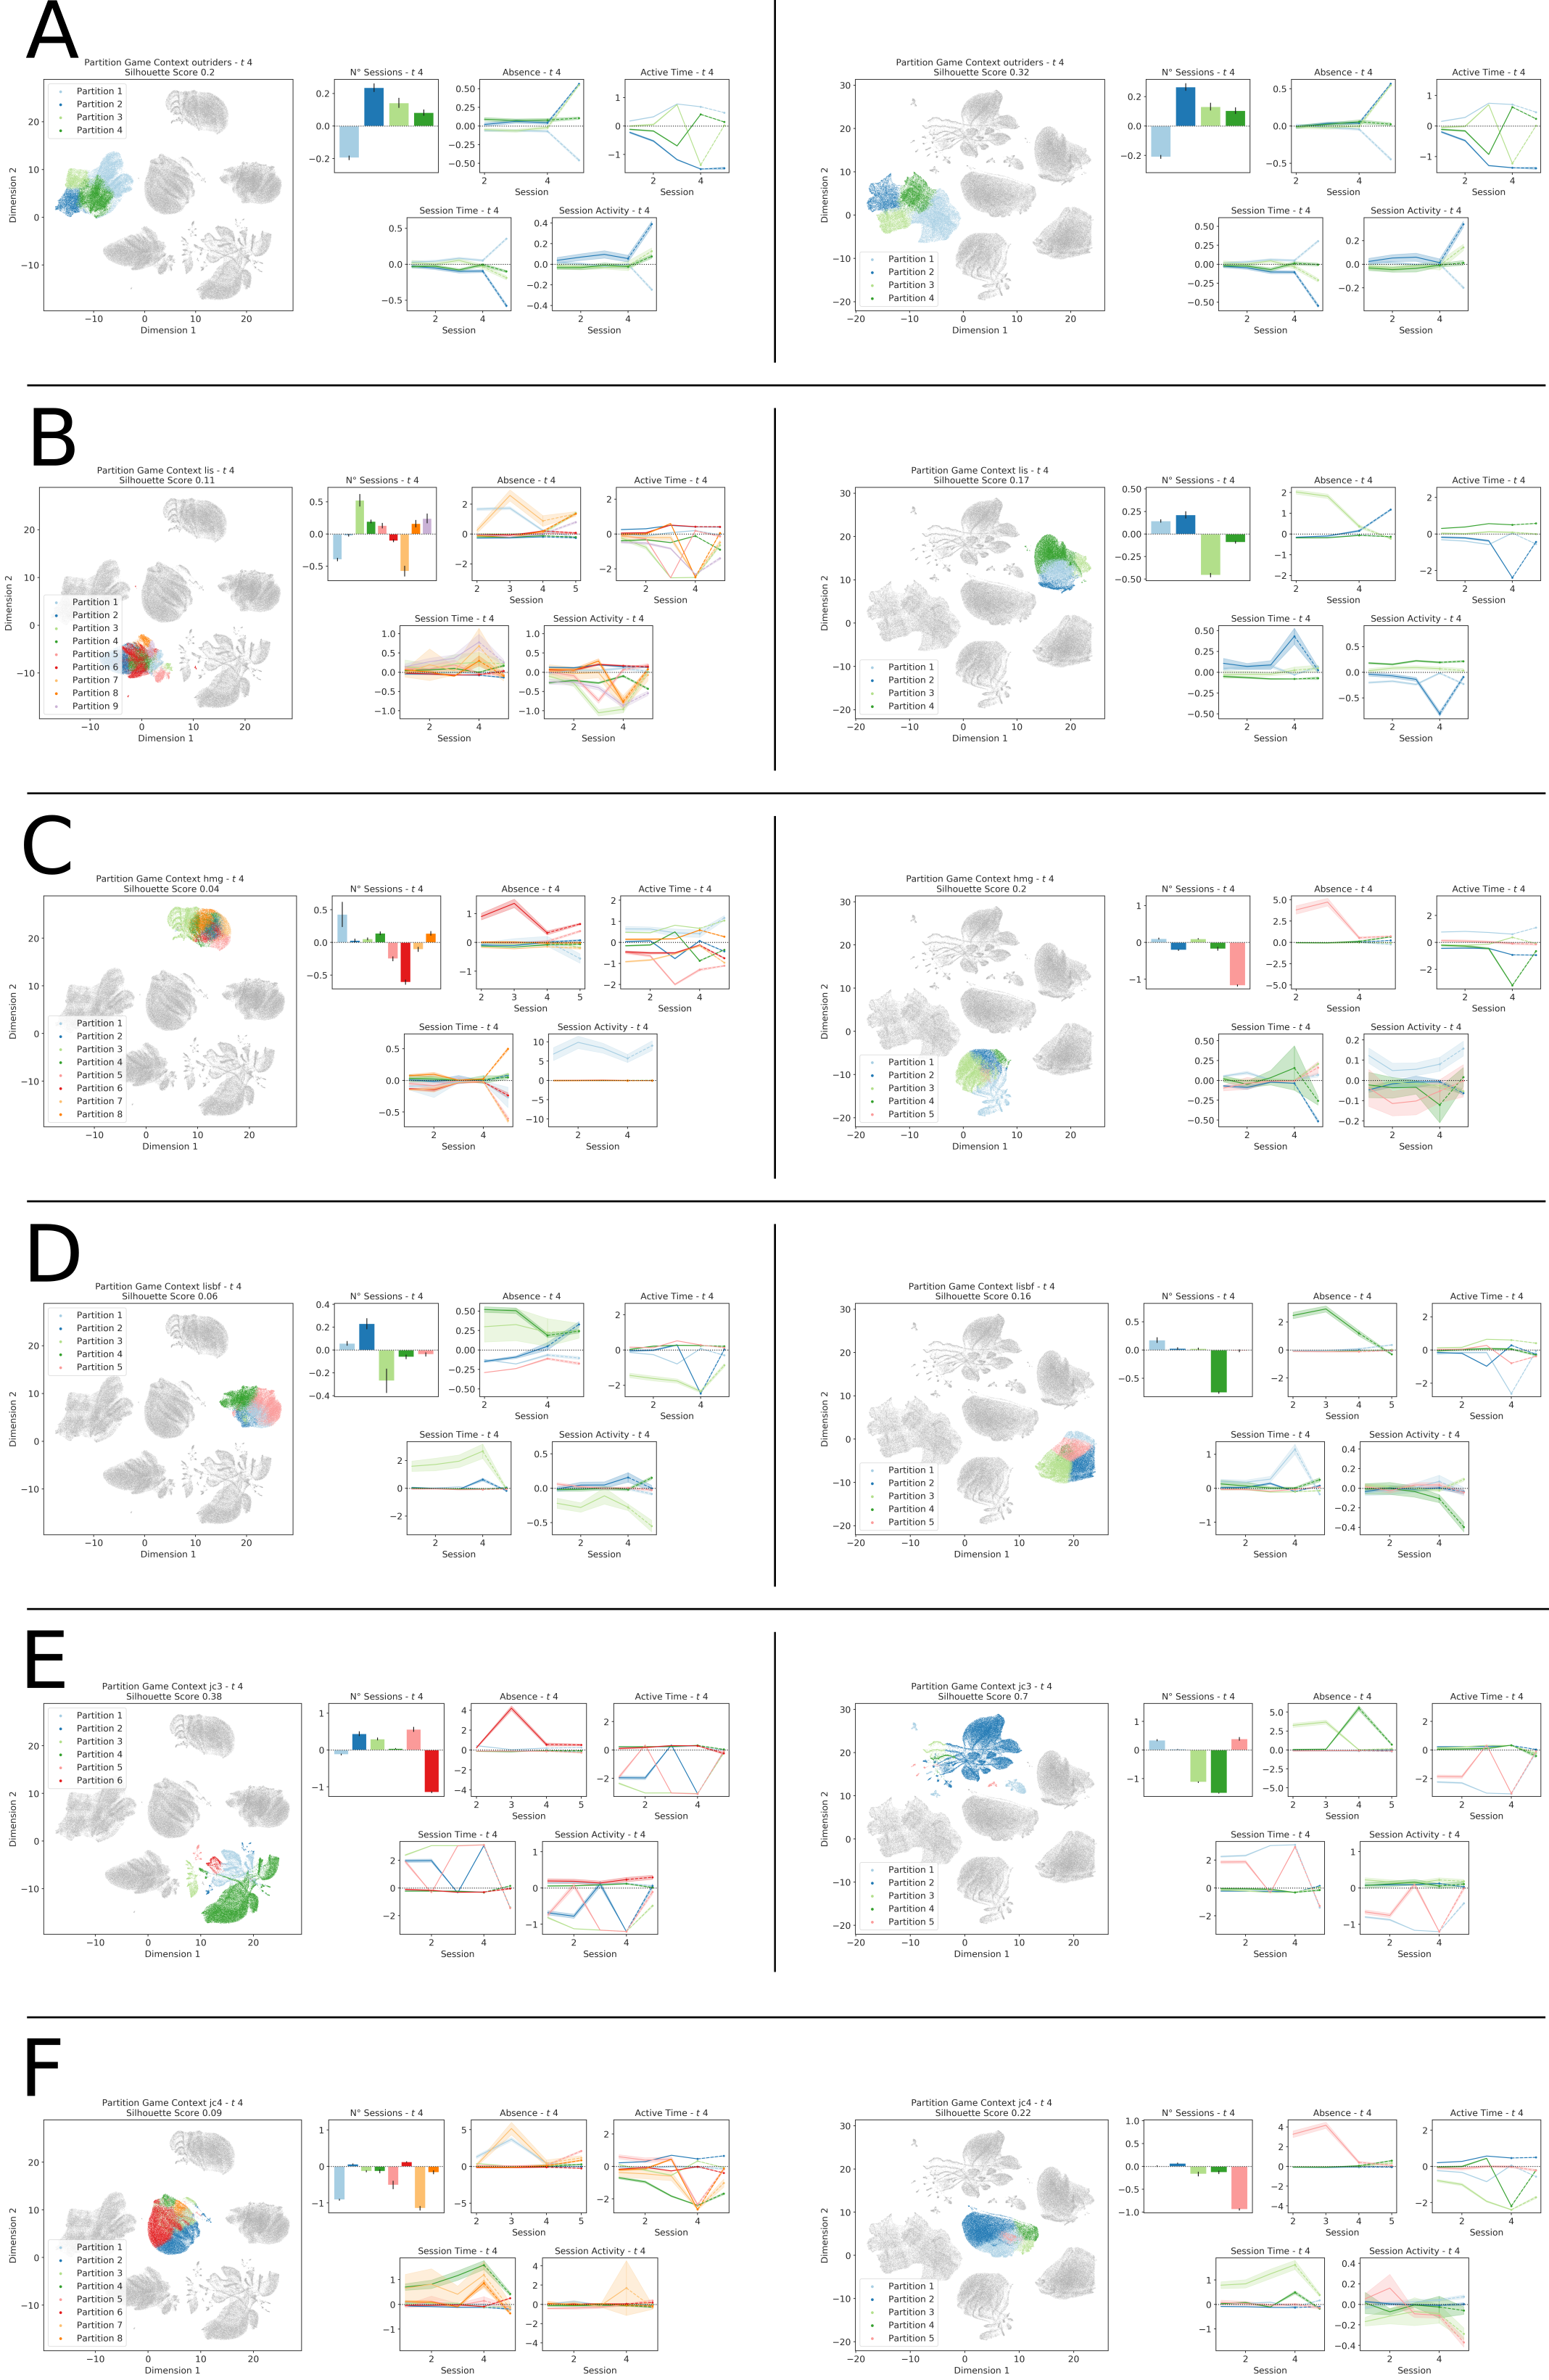
\includegraphics[width=0.7\textwidth]{images/appendix_D/clust_beha_all.png}
\centering
\caption[Partitions of the representations generated by the RNN architecture and its improved version from the behavioural metrics]{The two panels show the individuated partitions and associated profiles generated by applying Mini Batch KMeans to the representation generated by the RNN architecture and its improved version. All representations have been generated from the behavioural input.}
\label{partition_rnn_behaviour} 
\end{figure}
\FloatBarrier

\section{Partitions environmental metrics representations}
\label{partitions_environmental}

\subsection{Game Context hmg}
\label{env_clust_hmg}

\begin{figure}[ht]
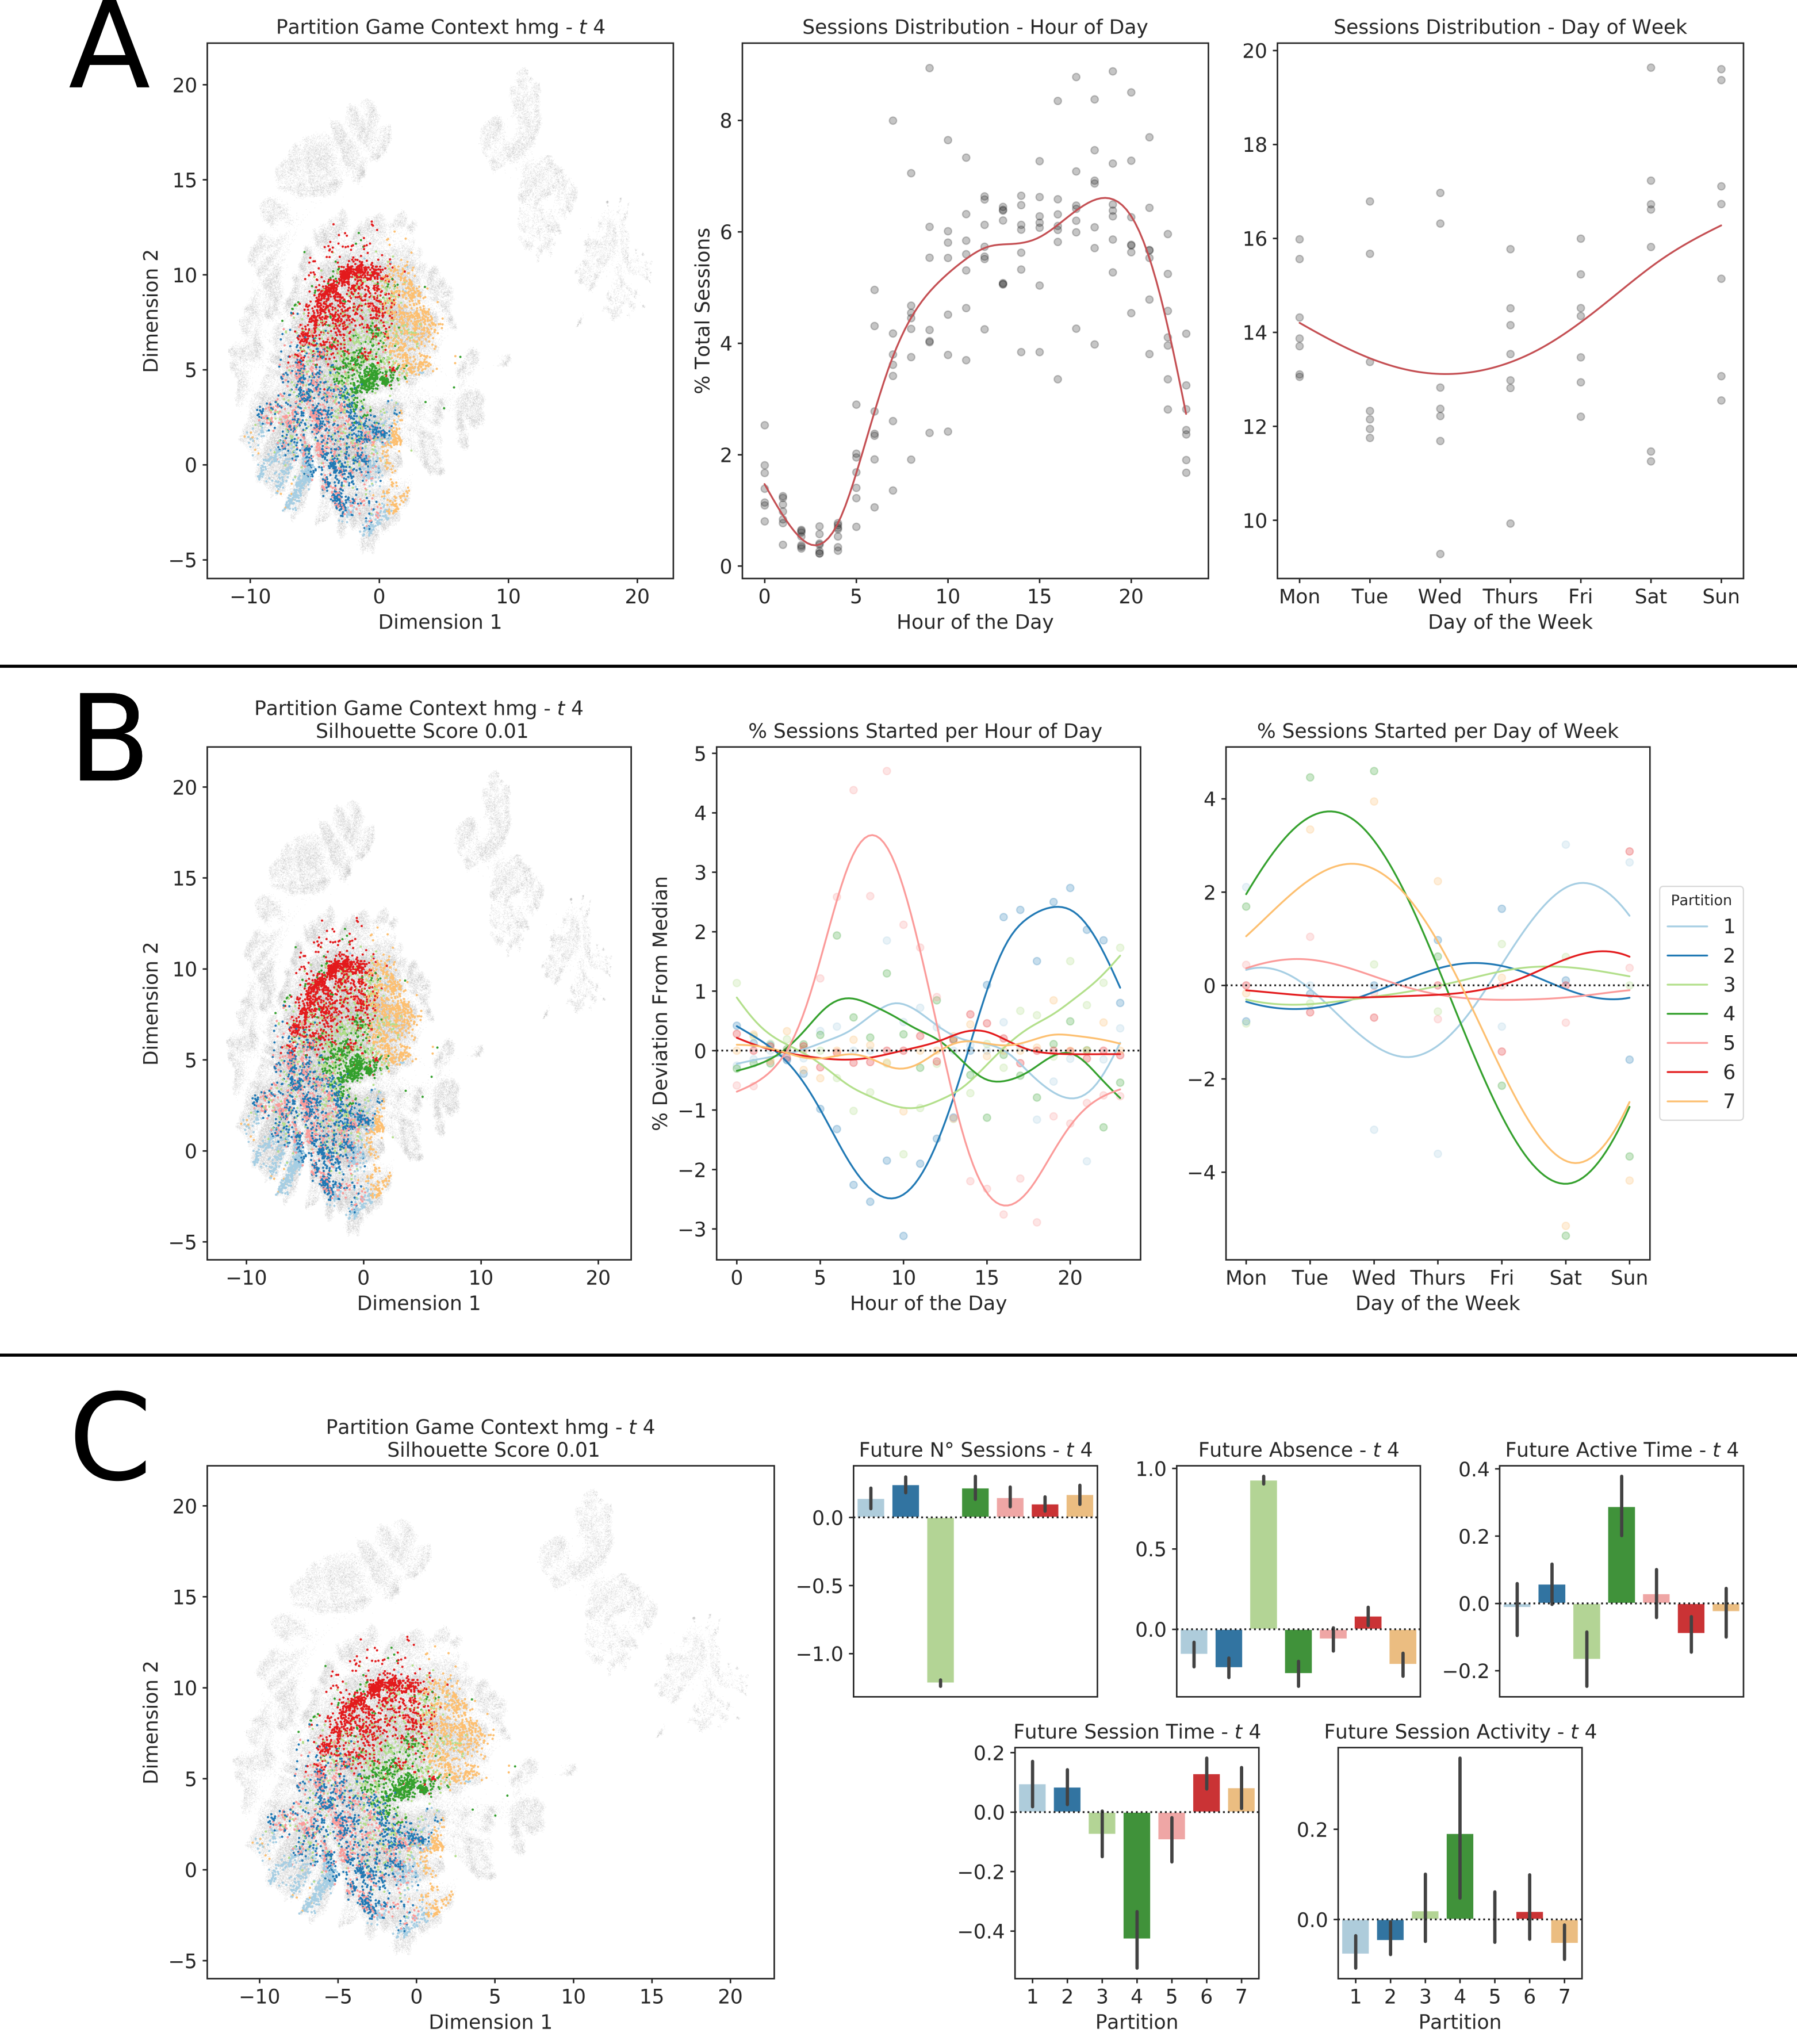
\includegraphics[width=0.7\textwidth]{images/appendix_D/clust_hmg_env.png}
\centering
\caption[Partitions of the representation generated from the environmental metrics for the game context hmg]{Partitions of the representation generated from the environmental metrics for the game context hmg}
\end{figure}
\FloatBarrier

\subsection{Game Context jc3}
\label{env_clust_jc3}

\begin{figure}[ht]
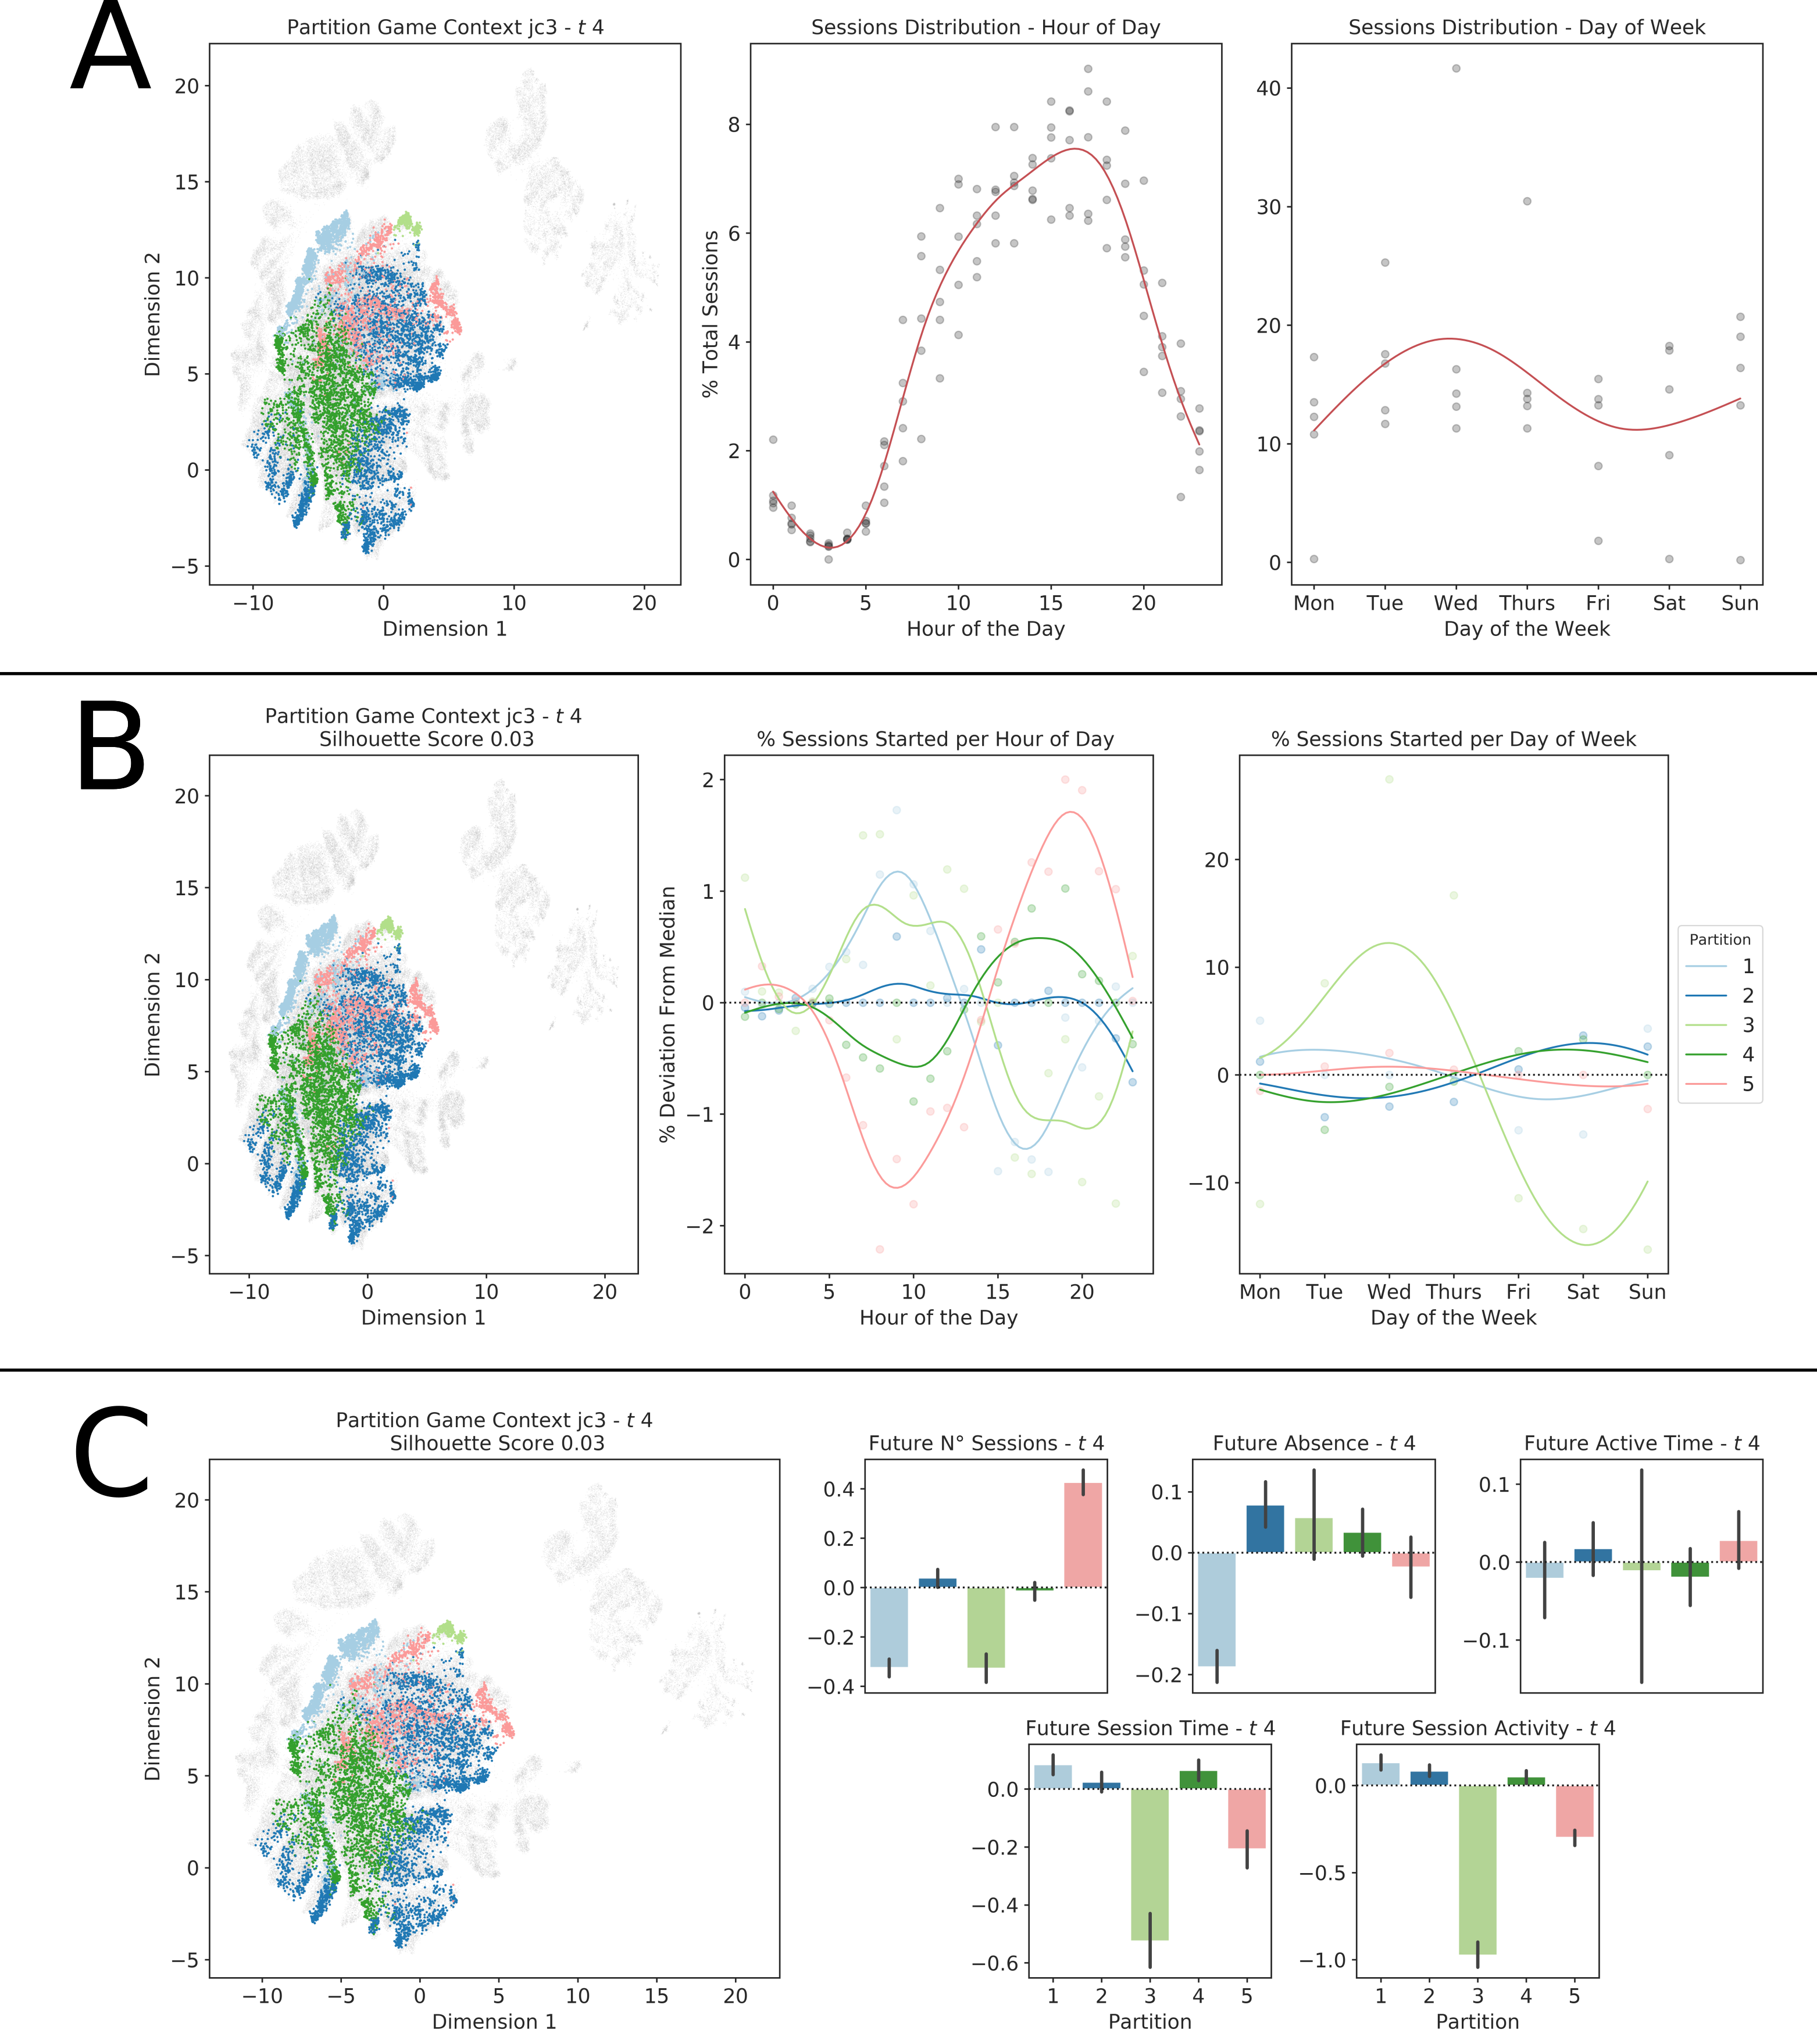
\includegraphics[width=0.7\textwidth]{images/appendix_D/clust_env_jc3.png}
\centering
\caption[Partitions of the representation generated from the environmental metrics for the game context jc3]{Partitions of the representation generated from the environmental metrics for the game context jc3}
\end{figure}
\FloatBarrier

\subsection{Game Context jc4}
\label{env_clust_jc4}

\begin{figure}[ht]
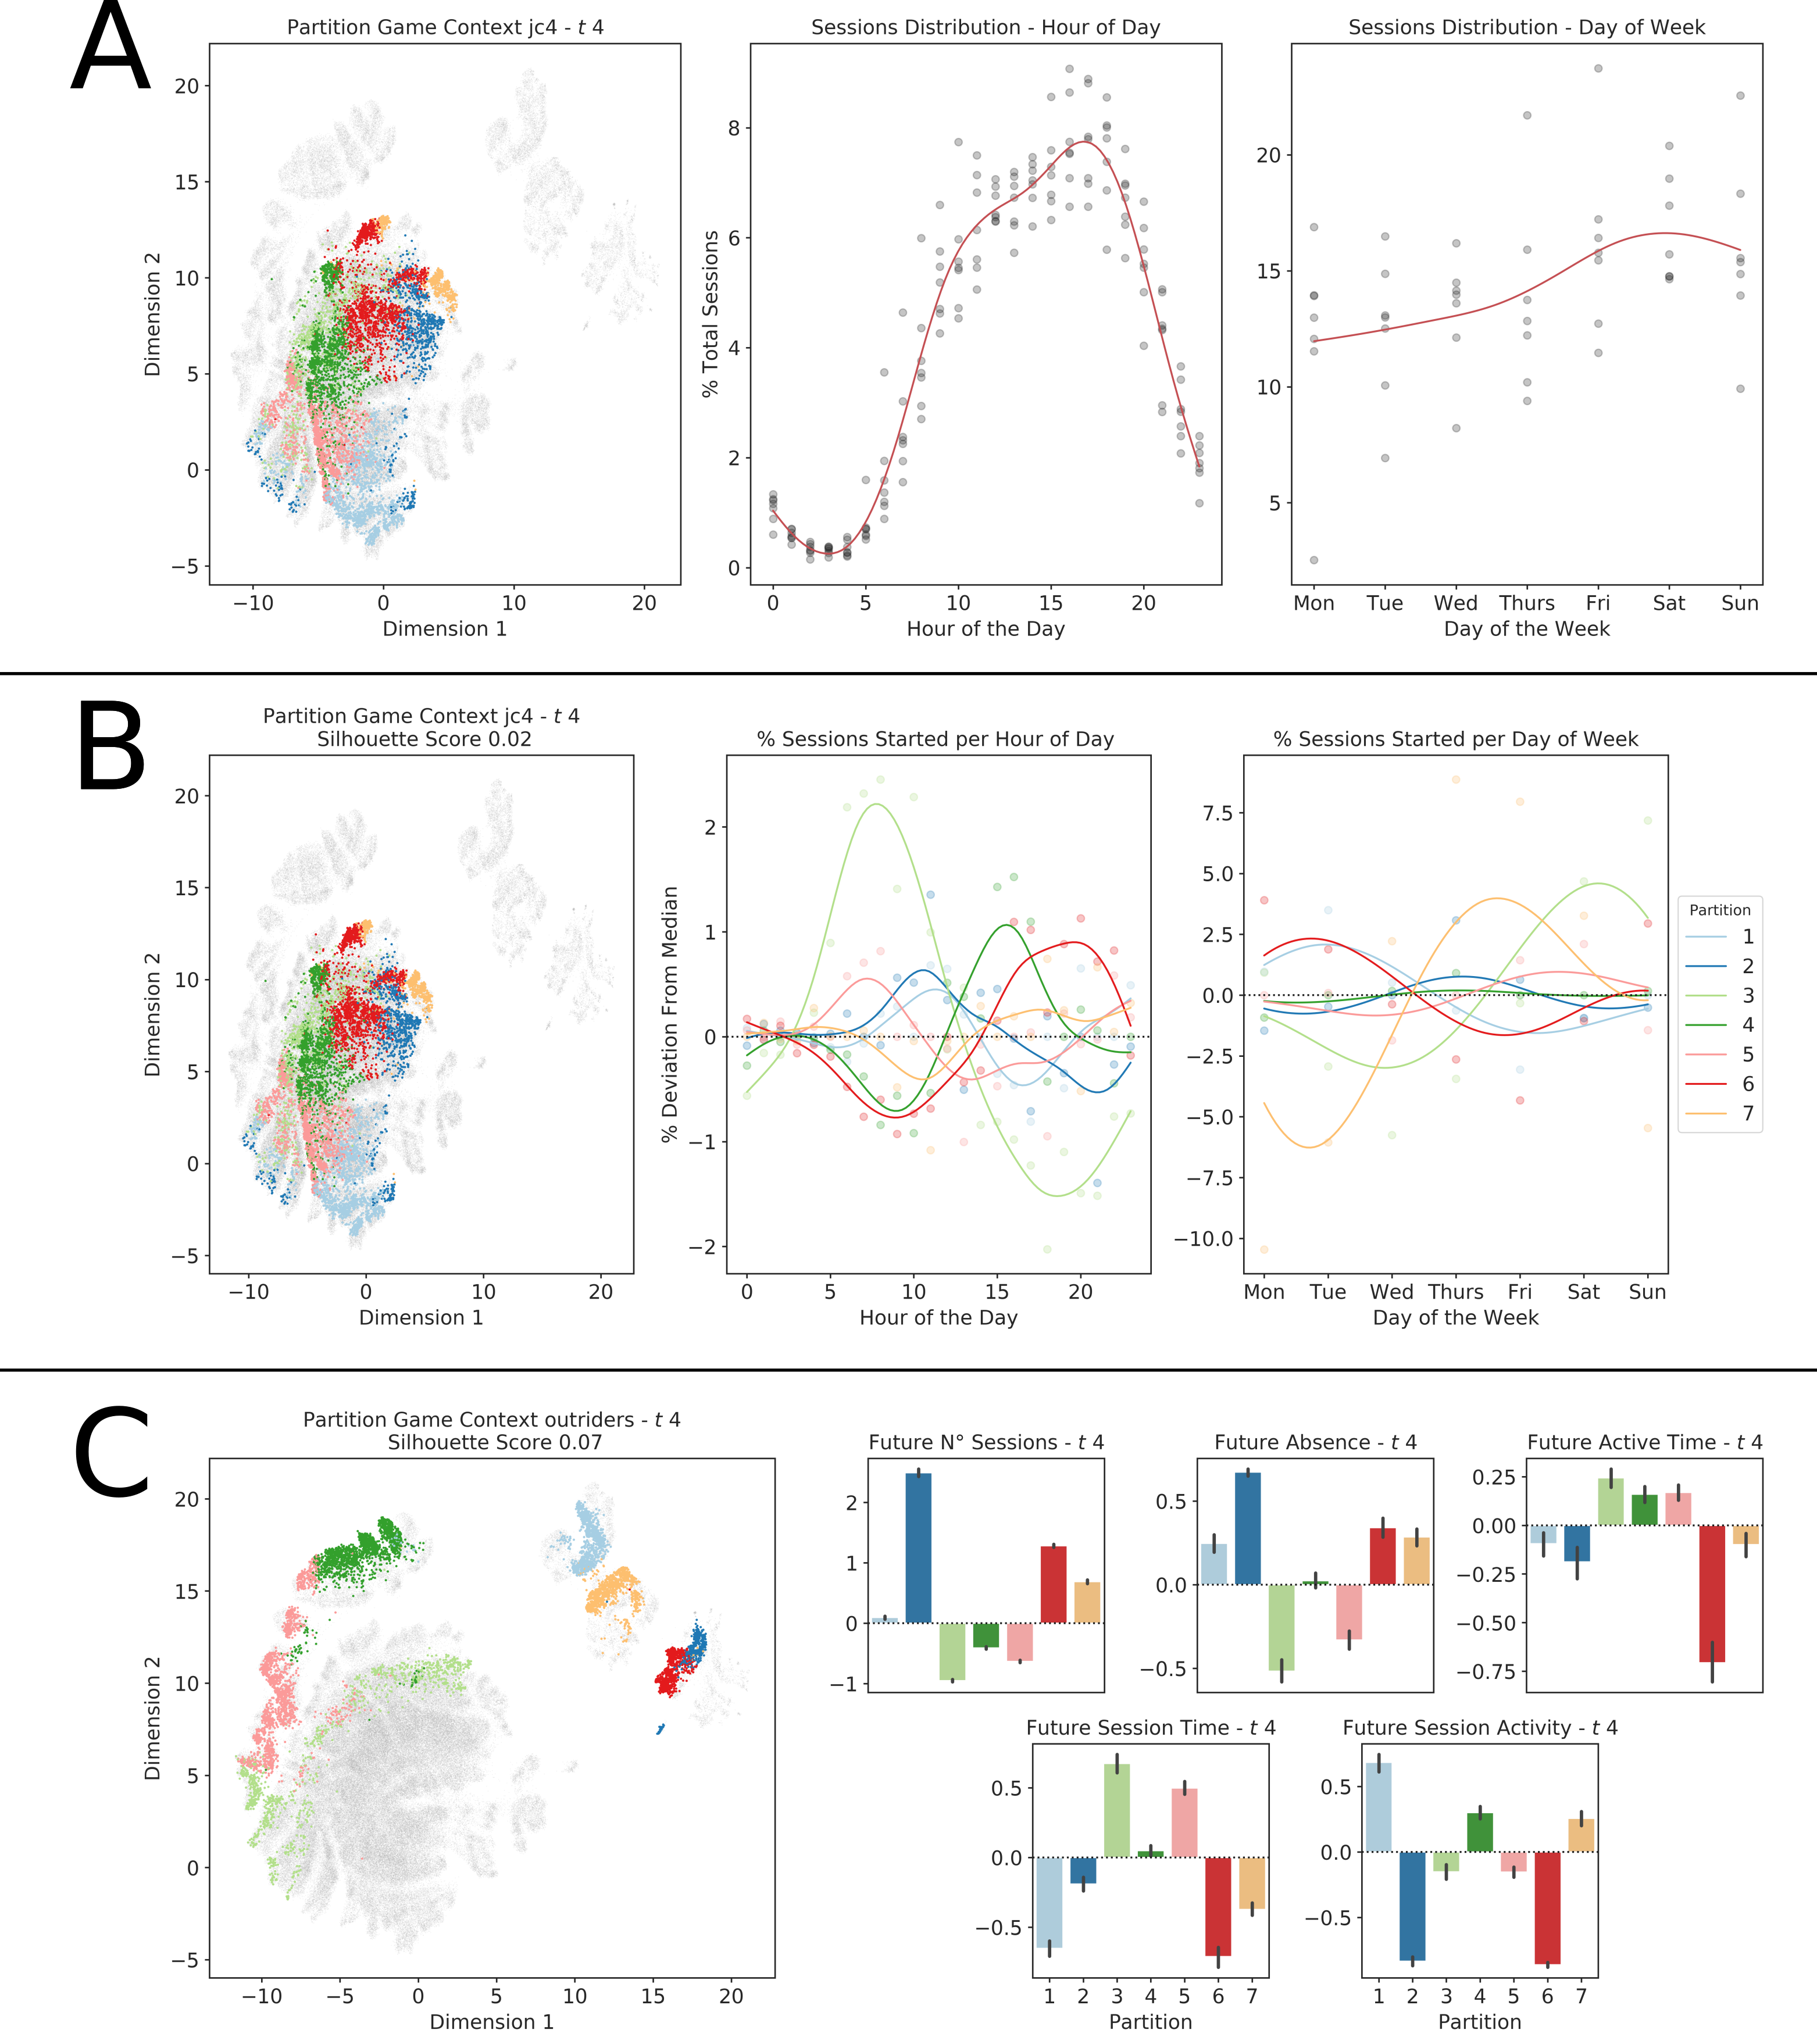
\includegraphics[width=0.7\textwidth]{images/appendix_D/clust_env_jc4.png}
\centering
\caption[Partitions of the representation generated from the environmental metrics for the game context jc4]{Partitions of the representation generated from the environmental metrics for the game context jc4}
\end{figure}
\FloatBarrier

\subsection{Game Context lis}
\label{env_clust_jc3}

\begin{figure}[ht]
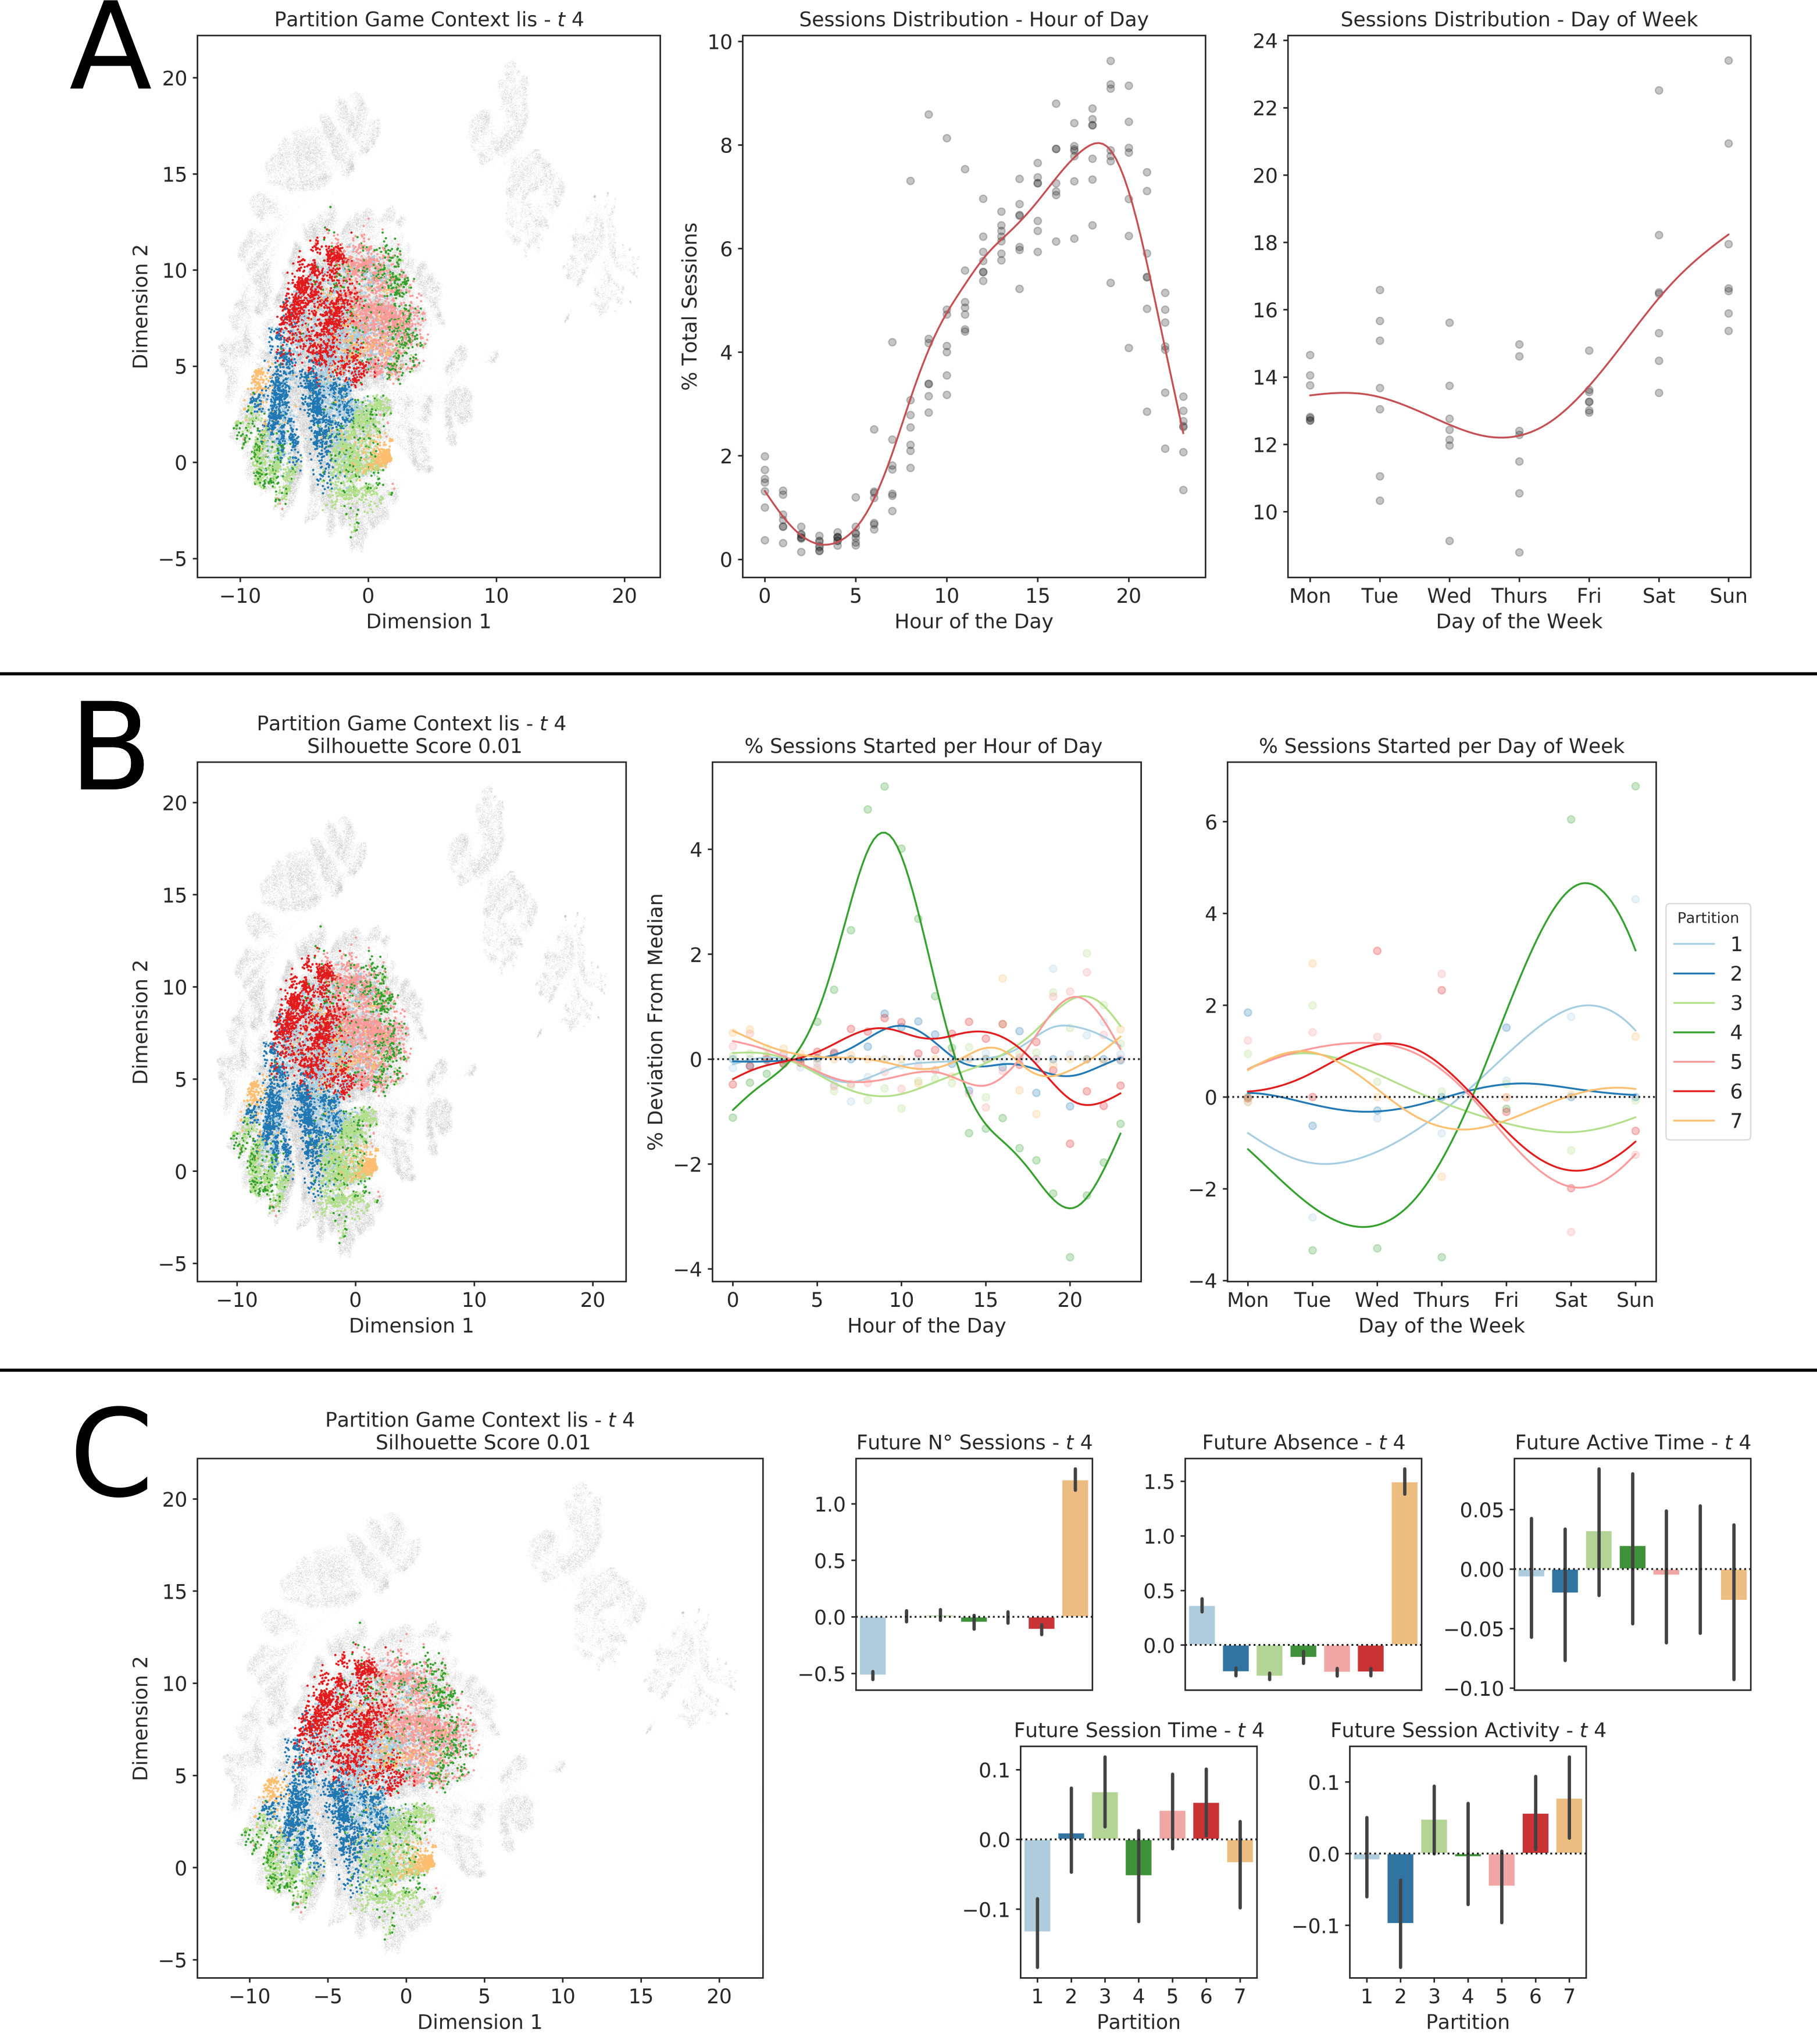
\includegraphics[width=0.7\textwidth]{images/appendix_D/clust_env_lis.png}
\centering
\caption[Partitions of the representation generated from the environmental metrics for the game context lis]{Partitions of the representation generated from the environmental metrics for the game context lis}
\end{figure}
\FloatBarrier

\subsection{Game Context lisbf}
\label{env_clust_lisbf}

\begin{figure}[ht]
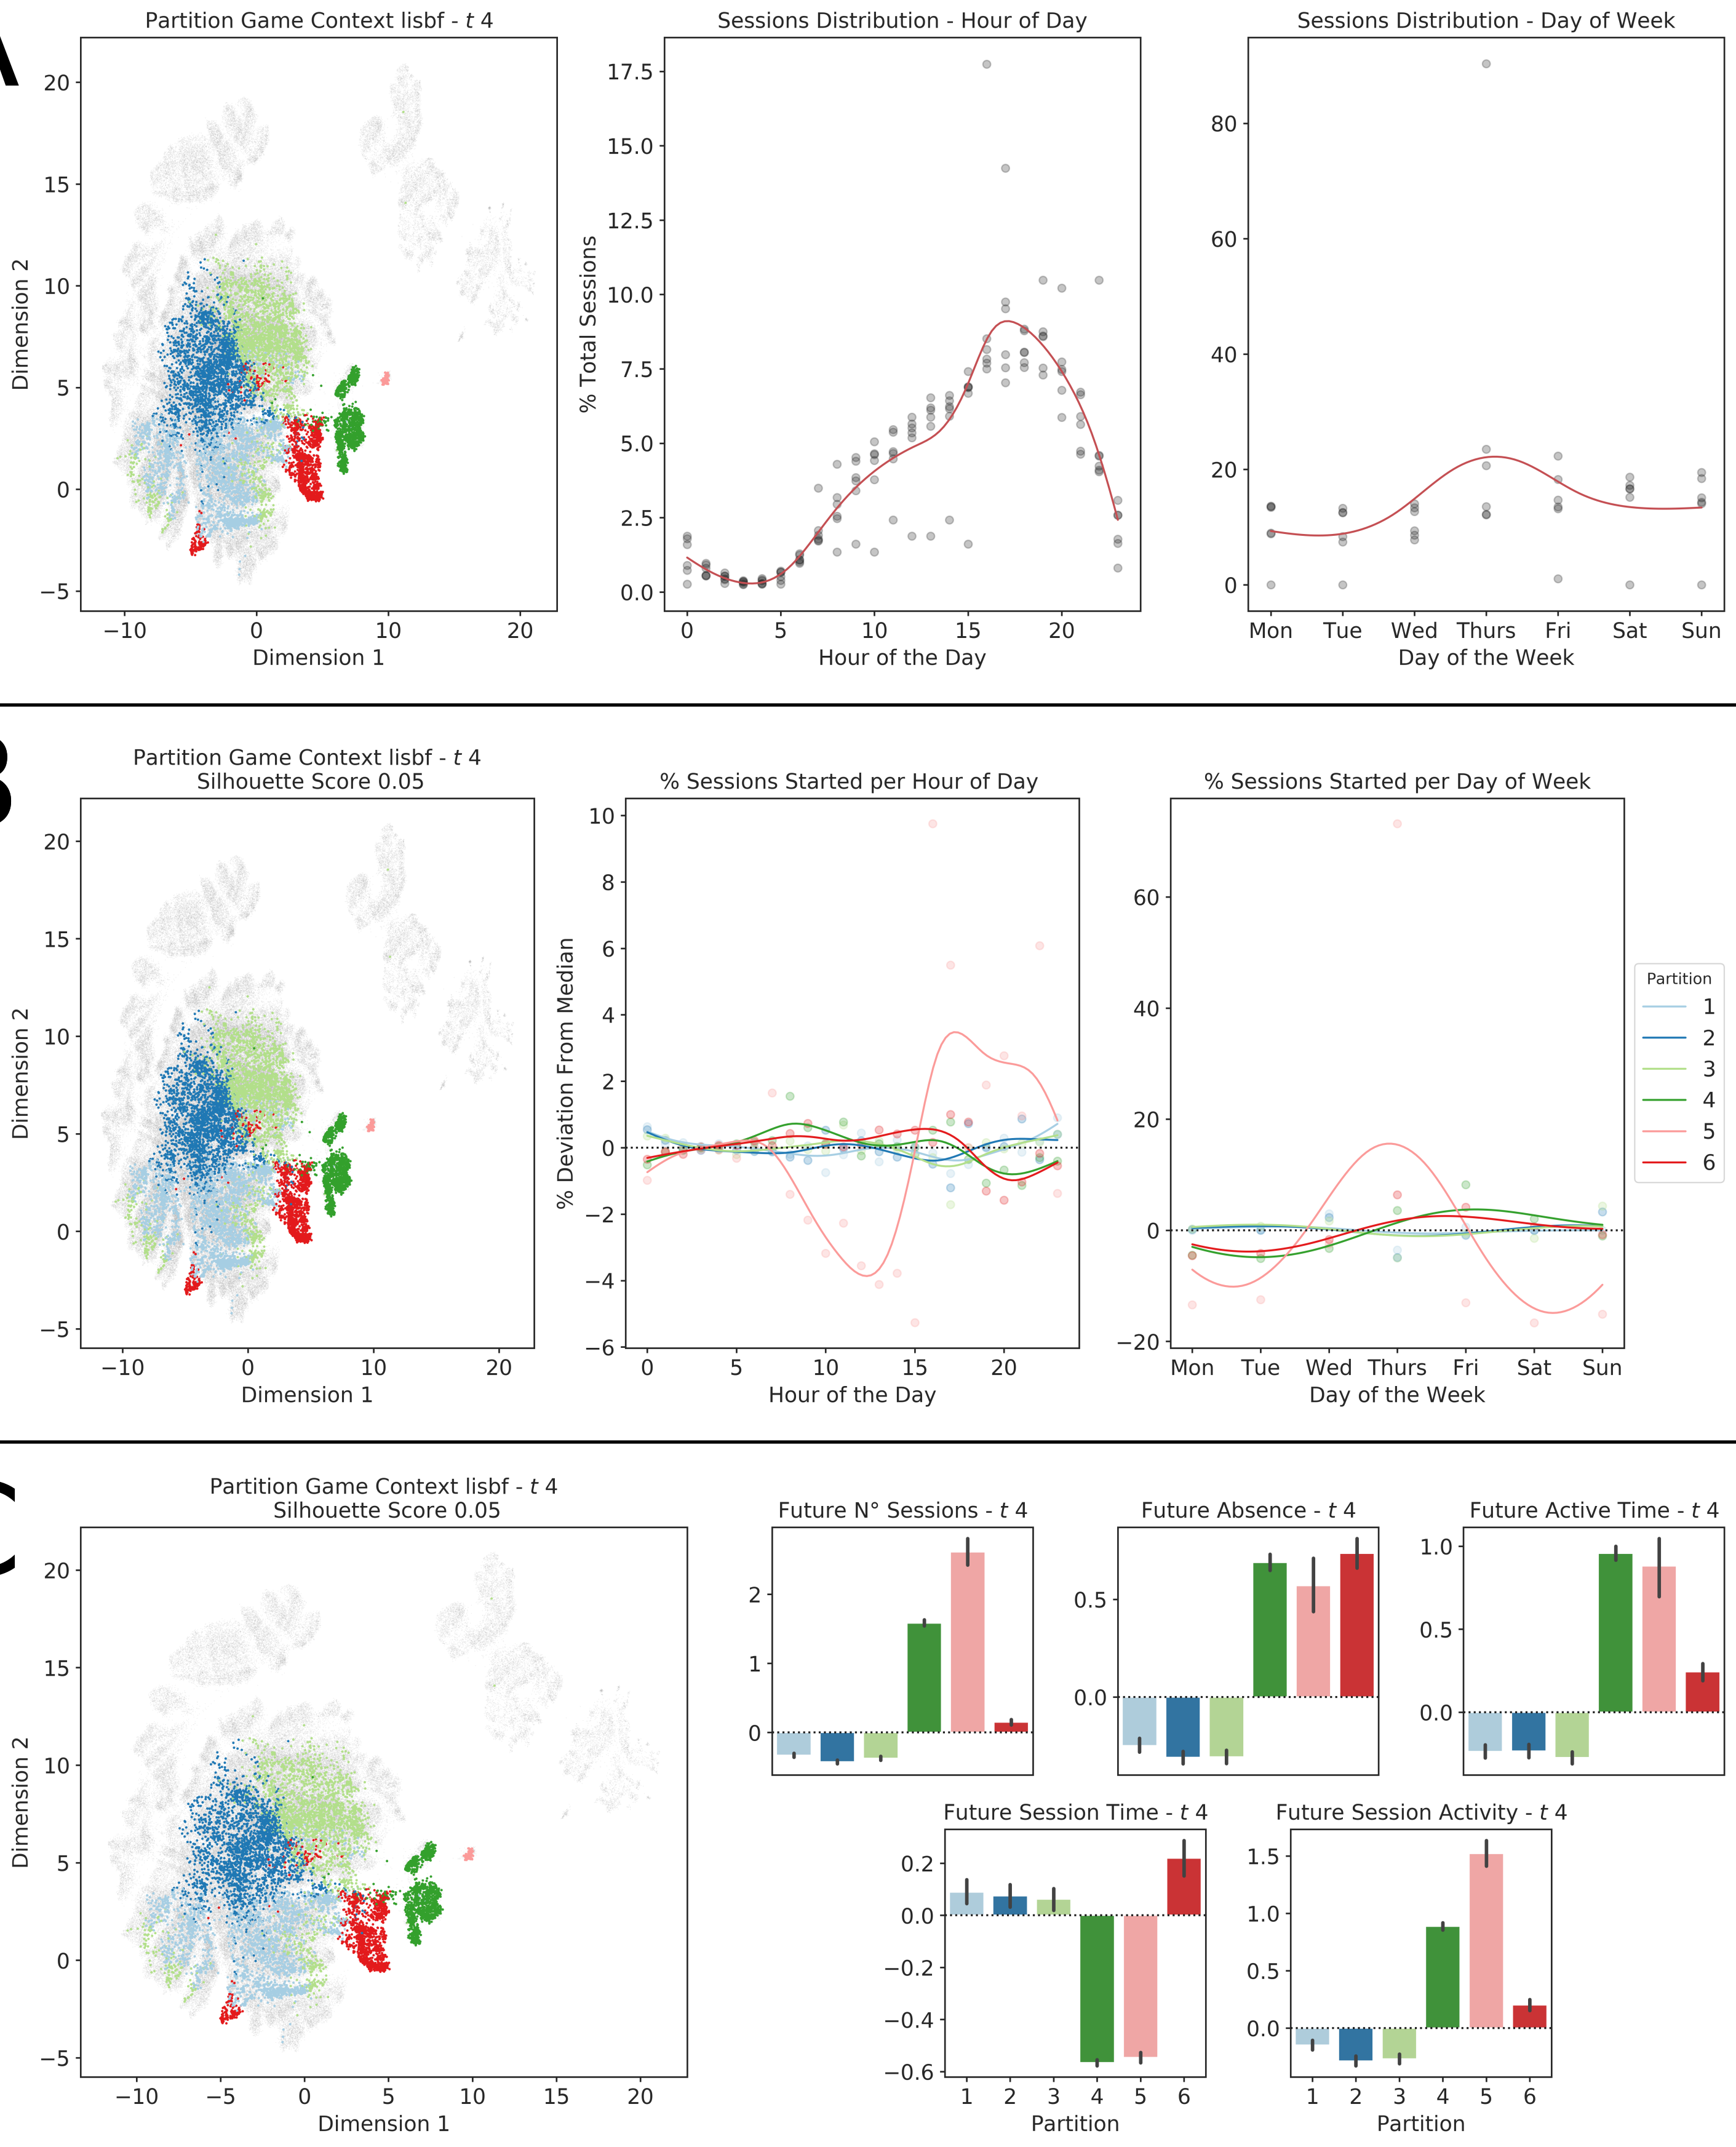
\includegraphics[width=0.7\textwidth]{images/appendix_D/clust_env_lisbf.png}
\centering
\caption[Partitions of the representation generated from the environmental metrics for the game context lisbf]{Partitions of the representation generated from the environmental metrics for the game context lisbf}
\end{figure}
\FloatBarrier

\section{Partitions game events metrics representations}
\label{partitions_game_events}